\documentclass{beamer}

\usepackage{mjclectureslides}

\definecolor{Dblue}{rgb}{.255,.41,.884}

\title[Limits and Continuity]
{Introduction to Analysis: \\ Limits and Continuity}
%\author[Prof. Michael Carlisle]{Prof. Michael Carlisle} 
%\institute{Baruch College, CUNY}
%\date{Fall 2017}
\date{}

\begin{document}

\frame{\titlepage}


\frame{ \frametitle{Limit of a Real-Valued Function at a Point}

\begin{defn}
Assume that a function 
\[ f: D \to \R \] 
is defined in a deleted neighborhood\footnote{$c$ is an accumulation point of $D$, but $c \in D$ is not necessary here.} of $c \in \R$, i.e. 

\[ \exists h > 0: \, N^*(c, h) \subseteq D. \]

\vspace{5mm}

The \textbf{limit} as $x$ approaches $c$ of the function $f$ is the value $L \in \R$, denoted
\[ \lim_{x \to c} f(x) = L, \]
if, the ``closer $x$ gets to $c$'', the ``closer $f(x)$ gets to $L$.''
\end{defn}

}


\frame{ \frametitle{Limit of a Real-Valued Function at a Point}

Formally: if 
\[ \forall \varepsilon > 0 \,\, \exists \delta = \delta(c, \ve) > 0: \,\, 0 < |x - c| < \delta \implies |f(x) - L| < \ve, \]
then we say 
\[ \lim_{x \to c} f(x) = L. \]

\vspace{5mm}

In neighborhood notation, 
\[ \forall \varepsilon > 0 \,\, \exists \delta > 0: \,\, x \in N^*(c, \delta) \implies f(x) \in N(L, \ve). \]

}


\frame{ \frametitle{Limits Bound Maps of Neighborhoods}

Restating the limit definition in neighborhood terms proves 

\vspace{5mm}

\begin{thm}
Suppose $f: D \to \R$ and let $c$ be an accumulation point of $D$. 

\vspace{5mm}

Then 
\[ \lim_{x \to c} f(x) = L \] 
if and only if, for each $\varepsilon > 0$ and neighborhood $V = N(L, \ve)$, 

\vspace{3mm}

$\exists \delta > 0$ and $U = N^*(c,\delta)$ such that the image 
\[ f(U \cap D) \subseteq V. \]
\end{thm}

}


\frame{ \frametitle{Limits Bound Maps of Neighborhoods}

Using $\ve = \frac{|L|}{2}$ in the definition of the limit proves 

\vspace{5mm}

\begin{cor} 
\textbf{(sign preservation near a nonzero limit)} 

\vspace{3mm}

Suppose $f: D \to \R$ and let $c$ be an accumulation point of $D$. \\
Suppose $\exists L > 0$ such that 
\[ \lim_{x \to c} f(x) = L. \] 
Then $\exists \delta > 0$ such that $0 < |x-c| < \delta \implies f(x) > 0$.
\end{cor}

}


\frame{ \frametitle{Sequential Criterion for Limits}

Here we relate limits of functions with convergence of sequences. 

\vspace{5mm}

\begin{thm} 
Suppose $f: D \to \R$ and let $c$ be an accumulation point of $D$. 

\vspace{5mm}

Then 
\[ \lim_{x \to c} f(x) = L \] 

\vspace{3mm}

iff for any sequence $(x_n)$ in $D \setminus \{c\}$, 
\[ \lim_{n \to \infty} x_n = c \implies \lim_{n \to \infty} f(x_n) = L. \] 
\end{thm}

}


\frame{ \frametitle{Sequential Criterion for Limits}

\pf $(\implies)$ Assuming 
\[ \lim_{x \to c} f(x) = L, \]
we need to show that, for any sequence $(x_n)$, 

\begin{center}
if $x_n \to c$, then $f(x_n) \to L$. 
\end{center}

\vspace{5mm}

We know that for each $\ve > 0$, 
\[ \exists \delta  > 0: \,\, 0 < |x - c| < \delta \implies |f(x) - L| < \ve. \]
If $x_n \to c$, 
\[ \exists N \in \N: \,\, \forall n > N, \,\, |x_n - c| < \delta. \]

}


\frame{ \frametitle{Sequential Criterion for Limits}

Then  
\[ |x_n - c| < \delta \implies |f(x_n) - L| < \ve, \]

\vspace{3mm}

which is precisely the criterion for $f(x_n) \to L$: for each $\ve > 0$, 
\[ \exists N \in \N: \,\, \forall n > N, \,\, |f(x_n) - L| < \ve. \]

\vspace{3mm}

($\Longleftarrow$) For this direction, a direct proof would be difficult. \\
Here, we use the contrapositive. To do so, we need to show 
\[ \lim_{x \to c} f(x) \neq L \implies(\exists (x_n): \, \lim_{n \to \infty} x_n = c  \text{ and } \lim_{n \to \infty} f(x_n) \neq L). \]

}


\frame{ \frametitle{Sequential Criterion for Limits}

Assume 
\[ \lim_{x \to c} f(x) \neq L. \]
Then $\exists \ve > 0$ such that 
\[ \forall \delta  > 0, \,\, \exists x \in D: \,\, 0 < |x - c| < \delta \text{ and } |f(x) - L| \geq \ve. \]

\vspace{3mm}

In particular, for each $n \in \N$, 
\[ \exists x_n \in D: \,\, |x_n - c| < \delta \text{ and } |f(x_n) - L| \geq \ve. \]

\vspace{3mm}

This gives us a sequence $(x_n)$ such that 
\[ \lim_{n \to \infty} x_n = c  \text{ and } \lim_{n \to \infty} f(x_n) \neq L. \,\,\,\, \blacksquare \]

}


% accumulation point implies unique limit
% no limit iff exists a sequence (s_n) \to c but f(s_n) does not converge
\frame{ \frametitle{Limits, if they exist, are unique}

\begin{cor}
If $f: D \to \R$, and $c$ is an accumulation point of $D$, \\
then if $f$ has a limit at $c$, the limit is unique.
\end{cor}

\vspace{5mm}

\begin{thm}
Suppose $f: D \to \R$, and $c$ is an accumulation point of $D$. \\
Then $f$ does not have a limit at $c$ iff \, $\exists$ a sequence $(x_n)$ in $D \setminus \{c\}$ such that $x_n \to c$ but $(f(x_n))$ does not converge in $\R$. 
\end{thm}

}


% examples
\frame{ \frametitle{Limits, if they exist, are unique}

\begin{ex}
$f(x) = \sin(\frac{1}{x})$ defined on $D = (0, \infty)$ has no limit at $x = 0$: consider the sequence $(x_n) = (\frac{2}{n\pi})$.
\end{ex}

\begin{figure}[!ht]
  \centering
    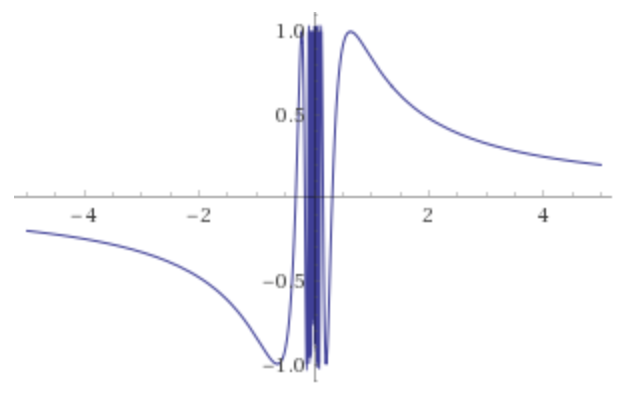
\includegraphics[width=3in]{sin1overx.png}
\end{figure}


}


% examples
\frame{ \frametitle{Limits, if they exist, are unique}

%\vspace{5mm}

\begin{ex}
The Dirichlet function
\[ f(x) = 1_{\Q}(x) = \left\{ \begin{array}{ll} 1 & x \in \Q \\ 0 & x \in \R \setminus \Q \end{array} \right. \]

\vspace{3mm}

has no limit at any $x \in \R$: for $c \in \R$, with decimal expansion $c = c_0.c_1 c_2 c_3 ...$, consider the sequence $(x_n)$ defined by 
\[ x_n = \left\{ \begin{array}{ll} c_0.c_1...c_n \in \Q & n \text{ even} \\ x_{n-1} + \frac{\sqrt{2}}{10^{n+1}} \in \R \setminus \Q  & n \text{ odd.} \end{array} \right. \]

\vspace{3mm}

Then $x_n \to c$ but $f(x_n) \not \to 0$ or 1.
\end{ex}

}


\frame{ \frametitle{Squeeze (Sandwich) Theorem}

\begin{thm} 
\textbf{(Squeeze Theorem)} Let $f, g, h$ be functions defined on a neighborhood $N(a,\ve)$ of $a$. 

\vspace{3mm}

If 
\[ \forall x \in N^*(a,\ve), \,\, f(x) \leq g(x) \leq h(x) \]
and 
\[ \lim_{x \to a} f(x) = \lim_{x \to a} h(x) = L. \]
Then 
\[ \lim_{x \to a} g(x) = L. \]
\end{thm}

}


\frame{ \frametitle{One-Sided Limits}

Note that the definition of a limit goes in ``both directions'': positive and negative. 

\vspace{3mm}

\begin{defn}
Assume that $f: D \to \R$ is a function, and $N^*(c, h) \subseteq D$ for some $h > 0$. The \textbf{one-sided limits} are defined as: 
\begin{align*} 
\textbf{left-hand limit}: & \lim_{x \to c-} f(x) = L \iff \\
 \forall \ve > 0, & \, \exists \delta_- > 0: \,\, - \delta_- < x - c < 0 \implies |f(x) - L| < \ve. \\
  & \\
\textbf{right-hand limit}: & \lim_{x \to c+} f(x) = L \iff \\
 \forall \ve > 0, & \, \exists \delta_+ > 0: \,\, 0 < x-c < \delta_+ \implies |f(x) - L| < \ve. 
 \end{align*}
\end{defn}

}

% limit properties: linearity, products, quotients... powers... polynomials... 
\frame{ \frametitle{One-Sided Limits}

The limit 
\[ \lim_{x \to c} f(x) = L, \]
only exists if 
\[  \lim_{x \to c-} f(x) = L =  \lim_{x \to c+} f(x). \]

\vspace{3mm}

There are several ways the limit may fail to exist: 
\begin{itemize}
\item Both one-sided limits exist, but do not match (jump)
\item One or both of the one-sided limits does not exist \\(vertical asymptote or oscillation). 
\end{itemize}

\vspace{3mm}

In either case we often use the notation DNE (``does not exist''): 
\[ \lim_{x \to c} f(x) \,\, DNE. \]

}


\frame{ \frametitle{Limits are Linear Maps}

Let $f, g: D \to \R$ be functions defined on a neighborhood of $c$, such that 
\[ \lim_{x \to c} f(x) = L, \,\, \lim_{x \to c} g(x) = M. \]

\vspace{5mm}

The limit is a \textbf{linear map}: for any $a, b \in \R$, 
\[ \lim_{x \to c} \left( a f(x) + b g(x) \right) = a \lim_{x \to c} f(x) + b \lim_{x \to c} g(x) = aL + bM. \]

}


\frame{ \frametitle{Limits are Linear Maps}

\pf We use an $\frac{\ve}{2}$-type argument. 

\vspace{5mm}

Since $f$ and $g$ have limits at $c$, then for any $\ve_f, \ve_g > 0$, $\exists \delta_f, \delta_g > 0$:

\[ |x - c| < \delta = \min(\delta_f, \delta_g) \implies |f(x) - L| < \ve_f, \, |g(x) - M| < \ve_g. \]

}


\frame{ \frametitle{Limits are Linear Maps}

Let $\ve > 0$ and choose $\ve_f$, $\ve_g > 0$ such that $\ve = |a| \ve_f + |b| \ve_g$. 

\vspace{5mm}

Then $\exists \delta = \min(\delta_f, \delta_g)$ (same as before) such that 

\begin{align*}
|x - c| < \delta \implies & \left|(a f(x) + b g(x)) - (aL + bM)\right| \\
 & \\
 & \leq \left|a f(x) - a L\right| + \left| b g(x) - bM\right| \\
 & \\
 & = |a| \cdot \left|f(x) - L\right| + |b| \cdot \left|g(x) - M\right| \\
 & \\
 & < |a| \ve_f + |b| \ve_g = \ve.  \,\,\,\, \blacksquare
\end{align*}

}


\frame{ \frametitle{Limits of Products, Quotients}

Products and quotients are also preserved by limits: 

\begin{align*} 
\lim_{x \to c} f(x) g(x) & = \left(\lim_{x \to c} f(x)\right) \left(\lim_{x \to c} g(x)\right) = LM, \\
 & \\
\lim_{x \to c} \frac{f(x)}{g(x)} & = \frac{\lim_{x \to c} f(x)}{\lim_{x \to c} g(x)} = \frac{L}{M} \,\, (\text{if } M \neq 0). 
\end{align*}

}


\frame{ \frametitle{Examples of Limits: Powers, Polynomials}

It should be clear from the linearity and product rules of limits that powers of $x$ have limits:  
\[ c \neq 0, \,\, n > 0 \implies \lim_{x \to c} x^n = c^n \]

From here it is easy to see that polynomials (with degree $n \in \N$) with real coefficients $a_i \in \R$, i.e. 
\[ p(x) = a_n x^n + a_{n-1} x^{n-1} + ... + a_1 x + a_0, \]

have limits for all $x \in \R$: 
\[ \lim_{x \to c} p(x) = a_n c^n + a_{n-1} c^{n-1} + ... + a_1 c + a_0. \]

}



\frame{ \frametitle{Examples of Limits}

\begin{ex}
\[ f(x) = \frac{x^2 + 2x - 5}{x^2 + 3x - 5} \implies \lim_{x \to 2} f(x) = \frac{3}{5}. \]
\end{ex}

\begin{ex}
\[ g(x) = \left\{ \begin{array}{ll} 3x^4 - x^2 + 3, & x > 1 \\ 26, & x = 1 \\ 5x, & x < 1 \end{array} \right.  \implies \lim_{x \to 1} g(x) = 5. \]
\end{ex}

}


% $\ve-\delta$ definition of continuity

\frame{ \frametitle{Continuity at a Point}

%We can generalize these properties in the notion of \emph{continuity}. 

\begin{defn}
A function $f: D \to \R$ defined at $c \in D$ is called \textbf{continuous at} $c$ if for any $\ve > 0$, 

\[ \exists \delta = \delta(c, \ve) > 0: \,\, |x-c| < \delta, \, x \in D \implies |f(x) - f(c)| < \ve. \]

\vspace{3mm}

This should look strikingly familiar to the definition of the limit of $f(x)$ as $x$ approaches $c$. 
\end{defn}

\vspace{5mm}

If this property is not met, $c$ is a \textbf{point of discontinuity} of $f$. 

\vspace{5mm}

If $f$ is continuous $\forall c \in S \subseteq D$, we call $f$ \textbf{continuous on} $S$, and \\if $f$ is continuous $\forall c \in D$, we call $f$ a \textbf{continuous function}. 

}


\frame{ \frametitle{Continuity at an Isolated Point is Automatic}

Note that, if $c$ is an isolated point of $D$ (not an accumulation point), then $f$ is trivially continuous at $c$ since $\exists \delta > 0$ such that $D$ contains no other points near $c$, i.e. 
\[ c \text{ isolated in } D \implies \exists \delta > 0: \,\, 0 < |x - c| < \delta \implies x \not \in D. \]

\begin{ex}
Let $D = (1,6) \cup \{8, 24.5, -3\}$. Then $f:D \to \R$ defined by 
\[ f(x) = 5x - 4 \] 
is a continuous function on $D$. 
\end{ex}

}

% thm: sequential criterion, nbhd criterion
\frame{ \frametitle{Sequential, Neighborhood Criteria of Continuity}

%Next, there are relationships between sequential convergence, neighborhoods, limits, and continuity: 
\begin{thm}
Let $f: D \to \R$ and $c \in D$. Then the following are equivalent: 
\begin{itemize}
\item[(a) ] $f$ is continuous at $c$. 
\item[(b) ] If $(x_n)$ is a sequence in $D$ such that $\lim_{n \to \infty} x_n = c$, then 
\[ \lim_{n \to \infty} f(x_n) = f\left(\lim_{n \to \infty} x_n\right) = f(c). \]
\item[(c) ] For any $\ve > 0$, 
\[ \exists \delta > 0: \,\, x \in N(c, \delta) \implies f(x) \in N(f(c), \ve). \]
\end{itemize}
Furthermore, if $c$ is an accumulation point of $D$, then (a)-(c) are all equivalent to 
\[ \lim_{x \to c} f(x) = f\left( \lim_{x \to c} x \right) = f(c). \]
\end{thm}

}



% eg: polynomials, etc
\frame{ \frametitle{Examples of Continuity: Powers, Polynomials}

It should be clear from the linearity and product rules of limits that powers of $x$ are continuous functions:  
\[ c \neq 0, \,\, n > 0 \implies \lim_{x \to c} x^n = c^n \]

From here it is easy to see that polynomials (with degree $n \in \N$) with real coefficients $a_i \in \R$, i.e. 
\[ p(x) = a_n x^n + a_{n-1} x^{n-1} + ... + a_1 x + a_0, \]

are continuous for all $x \in \R$: 
\[ \lim_{x \to c} p(x) = a_n c^n + a_{n-1} c^{n-1} + ... + a_1 c + a_0 = p(c). \]

}



\frame{ \frametitle{Examples of Continuity / Discontinuity}

\begin{ex}
\[ f(x) = \frac{x^2 + 2x - 5}{x^2 + 3x - 5} \implies \lim_{x \to 2} f(x) = \frac{3}{5} = f(2). \]
\end{ex}
Hence, $f$ is continuous at $x=2$. 

\begin{ex}
\[ g(x) = \left\{ \begin{array}{ll} 3x^4 - x^2 + 3, & x > 1 \\ 26, & x = 1 \\ 5x, & x < 1 \end{array} \right.  \implies \lim_{x \to 1} g(x) = 5 \neq g(1). \]
\end{ex}
Hence, $g$ is not continuous at $x=1$. 

}


\frame{ \frametitle{Examples of Continuity / Discontinuity}

\begin{ex}
%\[ f(x) = \left\{ \begin{array}{ll} x \sin(\frac{1}{x}) & x \neq 0 \\ 0 & x = 0 \end{array} \right. \]
Define $f(x) = x \sin(\frac{1}{x})$ if $x \neq 0$ and $f(0) = 0$. Then, for all $x \neq 0$, $f$ 
is continuous, and 
\[ |f(x) - f(0)| = \left|x \sin\left(\frac{1}{x}\right)\right| = \left|x\right| \left|\sin\left(\frac{1}{x}\right)\right| \leq |x| = |x-0|. \]
Hence, for any $\ve > 0$, the choice of $\delta = \ve$ satisfies 
\[ 0 < |x - 0| < \delta \implies |f(x) - f(0)| < \ve, \]
which proves that $f$ is continuous at $x=0$. 
\end{ex}

\vspace{5mm}

\begin{ex}
The Dirichlet function $1_{\Q}(x)$ has no limits for any $x \in \R$. Hence, it is discontinuous for every $x \in \R$. 
\end{ex}

}


\frame{ \frametitle{Different Types of Discontinuity}

There are many ways a function can be discontinuous at a point: 

\begin{itemize}
\item \textbf{removable jump discontinuity}: the limit value $L \in \R$, and 
\[ \lim_{x \to c} f(x) = L, \, \text{ but } f(c) \neq L. \] 
The function $f$ can be redefined at this point to make a continuous function: if $f$ has a removable jump at $c$, then 
\[ g(x) = \left\{\begin{array}{ll} f(x) & x \neq c \\ L & x = c \end{array}\right. \]
is continuous at $c$. 

\vspace{3mm}

\item \textbf{nonremovable jump discontinuity}: $\exists K, L \in \R$ such that 
\[ \lim_{x \to c+} f(x) = K \neq L = \lim_{x \to c-} f(x). \]
\end{itemize}

}


\frame{ \frametitle{Different Types of Discontinuity}

\begin{itemize}
\item $f$ is defined at $c$ (i.e. $f(c)$ exists), but $\lim_{x \to c} f(x)$ does not exist, due to \textbf{oscillations} of $f$ near $c$ \\(see, for example, $f(x) = \sin(\frac{1}{x})$ if $x \neq 0$, $f(0) = 0$). 

\vspace{3mm}

\item $f$ has a \textbf{vertical asymptote} at $x = c$:
\[ \lim_{x \to c+} f(x) = \infty \text{ or } -\infty, \,\, \text{ or } \lim_{x \to c-} f(x) = \infty \text{ or } -\infty. \]

\vspace{3mm}

\item If $f$ is undefined at $c$, then clearly $f$ cannot be continuous at $c$, even if the limit exists. \\
However, as with a removable jump discontinuity, if the limit exists, we can redefine the function at $c$ to be continuous.

\end{itemize}

}


% thm: discont iff sequential criterion breaks
% Dirichlet function, modified Dirichlet...
\frame{ \frametitle{Sequential Criterion of Discontinuity}

\begin{thm}
Let $f: D \to \R$ and $c \in D$. 

\vspace{5mm}

Then $f$ is discontinuous at $c$ iff $\exists$ a sequence $(x_n)$ in $D$ that converges to $c$ but $(f(x_n))$ does not converge to $f(c)$. 
\end{thm}

}


\frame{ \frametitle{Sequential Criterion of Discontinuity}

\begin{ex}
We modify the Dirichlet function to get a function that is continuous only at irrational values. Let
\[ f(x) = \left\{ \begin{array}{ll} \frac{1}{n} & x \in \Q, x = \frac{m}{n} \text{ in lowest terms} \\ 0 & x \in \R \setminus \Q. \end{array} \right. \]

If $c \in \Q$, a sequence $(x_n)$ of irrationals converging to $c$ \\(like, say, $x_n = \frac{\sqrt{2}}{n} + c$) all satisfy $f(x_n) = 0$, but $f(c) > 0$. 

\vspace{5mm}

Hence, $f$ is discontinuous at $c$. 

\vspace{5mm}

However, if $c \not \in \Q$, then any sequence $(x_n)$ converging to $c$ has $f(x_n) \to f(c) = 0$. Hence, $f$ is continuous at irrational $c$. 
\end{ex}

}


% properties: linearity, min, max, composition
\frame{ \frametitle{Linear Combos, Products, Quotients of Cont. Functions}

Let $f, g: D \to \R$ be continuous at $c$. Then: 

\vspace{3mm}

\begin{itemize}
\item Any linear combination of $f$ and $g$ is continuous at $c$, \\i.e. for any $a, b \in \R$, $af + bg$ is continuous at $c$. 

\vspace{3mm}

\item Products and quotients of continuous functions are also continuous: 

\begin{align*} 
\lim_{x \to c} f(x) g(x) & = \left(\lim_{x \to c} f(x)\right) \left(\lim_{x \to c} g(x)\right) = f(c) g(c), \\
 & \\
\lim_{x \to c} \frac{f(x)}{g(x)} & = \frac{\lim_{x \to c} f(x)}{\lim_{x \to c} g(x)} = \frac{f(c)}{g(c)} \,\, 
(\text{if } g(c) \neq 0). 
\end{align*}
\end{itemize} 

}


\frame{ \frametitle{Max, Min, Compositions of Cont. Functions}

Let $f, g: D \to \R$ be continuous at $c$. Then: 

\vspace{3mm}

\begin{itemize}
\item The maximum function $f \lor g(x) = \max(f, g)(x) = \max(f(x), g(x))$ and 

\vspace{3mm}

\item the minimum function $f \land g(x) = \min(f, g)(x) = \min(f(x), g(x))$ \\are both continuous. 

\vspace{3mm}

\item If $g$ is continuous on $D$ and $f$ is continuous on $g(D)$, \\then the composition $f \circ g(x) = f(g(x))$ is continuous on $D$. 
\end{itemize}

}


% thm: cont iff preimage of open is open
\frame{ \frametitle{Open Sets Determine Continuity}

The following theorem holds in the much more general setting of \emph{topological spaces}, not just in the special case of the real numbers.

\vspace{3mm}

\begin{thm}
$f:D \to \R$ is continuous on $D$ $\iff$ for every open set $G$ in $\R$ there exists an open set $H$ in $\R$ such that $H \cap D = f^{-1}(G)$. 
\end{thm}

\vspace{3mm}

\begin{cor}
$f: \R \to \R$ is continuous $\iff$ $f^{-1}(G)$ is open if $G$ is open. 
\end{cor}

}


\frame{ \frametitle{Bounded Functions}

\begin{defn}
$f: D \to \R$ is called a \textbf{bounded function} if $\exists M > 0$ such that 
\[ \forall x \in D, \, |f(x)| \leq M, \]
i.e. the range $f(D) \subseteq \R$ is a bounded set. 
\end{defn}

\vspace{3mm}

\begin{notenote}
$D$ bounded does not imply $f(D)$ bounded. \\
Try $f:(0,1) \to \R$ defined by $f(x) = \frac{1}{x}$. 
\end{notenote}

\vspace{3mm}

% thm: D compact, f cont --> f(D) compact
\begin{thm} % Thm II
%Suppose $f$ is continuous on $[a,b]$. Then $f$ is bounded on $[a,b]$. 
$f: D \to \R$ is continuous, and $D$ is compact $\implies$ $f(D)$ is compact.
\end{thm}

}

\frame{ \frametitle{Continuous image of a compact set is compact}

\begin{thm} 
$f: D \to \R$ is continuous, and $D$ is compact $\implies$ $f(D)$ is compact.
\end{thm}

\vspace{5mm}

\pf Let $\mc{G} = \{G_\alpha\}$ be an open cover of $f(D)$. 

\vspace{3mm}

We will show that $\mc{G}$ has a finite subcover. 

\vspace{3mm}

By the previous theorem, since $f$ is continuous on $D$, we have that 
\[ \text{for each } G_{\alpha} \in \mc{G}, \exists H_{\alpha} \subseteq \R \text{ open such that } H_{\alpha} \cap D = f^{-1}(G_{\alpha}). \]

}


\frame{ \frametitle{Continuous image of a compact set is compact}

Since $f(D) \subseteq \bigcup_{\alpha} G_{\alpha}$, it follows that 

\[ D \subseteq \bigcup_{\alpha} f^{-1}(G_{\alpha}) \subseteq \bigcup_{\alpha} H_{\alpha}. \]

\vspace{3mm}

Thus, the collection $\{H_{\alpha}\}$ is an open cover of $D$. 

\vspace{3mm}

$D$ is compact, so there is a finite subcover 
\[ \{H_{\alpha_1}, H_{\alpha_2}, ..., H_{\alpha_n}\} \] 

such that 
\[ D \subseteq \bigcup_{i=1}^n H_{\alpha_i}. \]

}


\frame{ \frametitle{Continuous image of a compact set is compact}

Note that 
\begin{align*} 
D \subseteq \bigcup_{i=1}^n H_{\alpha_i} & \implies D \subseteq \bigcup_{i=1}^n (H_{\alpha_i} \cap D) \implies f(D) \subseteq \bigcup_{i=1}^n G_{\alpha_i}. 
\end{align*}

Hence, $\{G_{\alpha_i}\}_{i=1}^n$ is a finite subcover of $\mc{G}$ for $f(D)$. 

\vspace{3mm}

 $\therefore$ $f(D)$ is compact. \,\, $\blacksquare$

}


% cor: D compact, f cont --> f assumes max and min (EVT)
\frame{ \frametitle{The Attainment of Extreme Values}

As a corollary we get the well-known
\begin{cor} 
\textbf{Extreme Value Theorem (EVT)} Let $f$ be continuous on $[a,b]$. 

\vspace{3mm}

Then $f$ attains its minimum (greatest lower bound, infimum) and maximum (least upper bound, supremum) on $[a,b]$. 
\end{cor}

\vspace{5mm}

\pf $f$ is continuous on $[a,b]$, and $[a,b]$ is compact, so the image $f([a,b])$ is compact. 
Thus, $f([a,b])$ contains its min and max:

\vspace{5mm}

$\exists x_m$, $x_M$ $\in [a,b]$ and $m, M \in f([a,b])$ such that 
\[ \forall x \in [a,b], \,\, f(x_m) = m \leq f(x) \leq M = f(x_M). \,\, \blacksquare \]

}


\frame{ \frametitle{Sign Preservation}

\begin{thm} 
\textbf{(Sign Preservation)} Let $f:[a,b] \to \R$ be continuous, $c \in (a,b)$. 

\vspace{5mm}

Then, if $f(c) \neq 0$, $\exists$ a neighborhood $N = N(c,\ve)$ of $c$ such that 
\[ \forall x \in N(c, \ve), \,\, f(x) \text{ and } f(c) \text{ have the same sign. } \]
\end{thm}

}


\frame{ \frametitle{Sign Preservation}

\pf WLOG assume $f(c) > 0$. 

\vspace{5mm}

Since $f$ is continuous at $c$, and $f(c) = y_0 > 0$, then for any $\ve > 0$, 
\[ \exists \delta > 0: \,\, 0 < |x - c| < \delta \implies |f(x) - y_0| < \ve. \]

\vspace{3mm}

Choosing $\ve = \frac{y_0}{2} > 0$, we get some $\delta > 0$ such that 
\[ x \in (c - \delta, c + \delta) \implies f(x) \in \left(\frac{y_0}{2}, \frac{3y_0}{2}\right). \,\, \therefore \, f(x) > 0. \]

\vspace{3mm}

If $f(c) < 0$, consider $g(x) = -f(x)$. \,\, $\blacksquare$

}


% lemma: f cont, hits both sides of 0 --> hits 0
\frame{ \frametitle{The Intermediate Value Theorem (version 0)}

\begin{lemma} 
\textbf{Intermediate Value Theorem (IVT) (through 0)} \\
Suppose $f$ is continuous on $[a,b]$, and that $f(a) < 0 < f(b)$. 

\vspace{5mm}

Then $\exists c \in (a,b)$ such that $f(c) = 0$.
\end{lemma}

\vspace{5mm}

\pf Let\footnote{In pre-image terms, $S = [a,b] \cap f^{-1}((-\infty, 0])$.} 
\[ S = \{x \in [a,b]: \,\, f(x) \leq 0\}. \]

\vspace{3mm}

Let $c = \sup S$. We claim that $f(c) = 0$. 

}


% lemma: f cont, hits both sides of 0 --> hits 0
\frame{ \frametitle{The Intermediate Value Theorem (version 0)}

For a contradiction, suppose that $f(c) < 0$. 

\vspace{5mm}

Then, by sign preservation, $\exists$ a neighborhood $U$ of $c$ such that 
\[ \forall x \in U \cap [a,b], \, f(x) < 0. \]

\vspace{3mm}

Since $f(c) < 0 < f(b)$, $\exists p \in U$ such that $c < p < b$. \\

\vspace{5mm}

But $f(p) < 0$ since $p \in U$. 

\vspace{5mm}

Thus, $p \in S$, which contradicts $c = \sup S$. $\contra$ \,\, $\therefore$ $f(c) \geq 0$. 

}


\frame{ \frametitle{The Intermediate Value Theorem (version 0)}

Likewise, suppose for another contradiction that $f(c) > 0$. 

\vspace{5mm}

Then, again by sign preservation, $\exists V = V(c, \ve)$ for some $\ve > 0$:
\[ \forall x \in V \cap [a,b], \, f(x) > 0. \]

\vspace{3mm}

Then, since $f(a) < 0 < f(c)$, $\exists q \in V$ such that $a < q < c$. 

\vspace{5mm}

Hence, $f(q) > 0$, and so $q$ is an upper bound for $S$ with $q < c$, contradicting $c = \sup S$. $\contra$ \,\, $\therefore$ $f(c) \leq 0$. 

\vspace{5mm}

Therefore, $f(c) = 0$, and $c \neq a$ and $c \neq b$ $\implies c \in (a,b)$. \,\, $\blacksquare$

}


% thm: IVT
\frame{ \frametitle{The Intermediate Value Theorem}

\begin{thm} 
\textbf{Intermediate Value Theorem (IVT)} \\
Suppose $f$ is continuous on $[a,b]$, and that $f(a) \neq f(b)$. 

\vspace{5mm}

Then, as $x$ varies from $a$ to $b$, $f(x)$ takes on every value $k$ between $f(a)$ and $f(b)$. 
\end{thm}

\vspace{5mm}

\textbf{Intuition} If $f$ is continuous on $[a,b]$, you don't need to lift your pencil when drawing the graph of $f$. 

\vspace{5mm}

In addition, every horizontal line $y=k$ for $k$ between $f(a)$ and $f(b)$ crosses the graph at least once.

}


\frame{ \frametitle{The Intermediate Value Theorem}

\pf WLOG, assume $f(a) < f(b)$. We show 
\[ \forall k \in (f(a), f(b)), \, \exists x_k \in (a,b): \, f(x_k) = k. \]

\vspace{3mm}

Apply the previous lemma to the continuous function 
\[ g(x) = f(x) - k, \]
since 
\[ g(a) = f(a) - k < 0 \text{ and } g(b) = f(b) - k > 0.\]

\vspace{3mm}

Thus $\exists c \in (a,b)$ such that 
\[ g(c) = f(c) - k = 0 \implies f(c) = k. \]

The $f(a) > f(b)$ case repeats the argument on $h(x) = -g(x)$. \,\, $\blacksquare$

}


% f cont on compact interval I --> f(I) is a compact interval
\frame{ \frametitle{Cont. image of a compact interval is a compact interval}

We now refine the theorem from the beginning of the section:

\vspace{5mm}

\begin{thm} 
Suppose $f$ is continuous on $[a,b]$. Then $f$ is bounded on $[a,b]$. 
\end{thm}

\vspace{5mm}

can be focused to the more immediately-applicable 

\vspace{5mm}

\begin{thm} 
Suppose $f: D \to \R$ is continuous, and $D$ is a compact interval. \\Then $f(D)$ is a compact interval.
\end{thm}

}


\frame{ \frametitle{Cont. image of a compact interval is a compact interval}

\pf Since $D$ is compact and $f$ is continuous, \\by the EVT $f(D)$ attains its min $m$ and max $M$. 

\vspace{3mm}

Thus, $f(D) \subseteq [m,M]$, and 
\[ \exists x_m, x_M \in D: \, f(x_m) = m, \, f(x_M) = M. \]

If $m = M$, then $f$ is a constant function and we are done.

\vspace{3mm}

Else, $m < M$. Clearly, $m, M \in f(D)$. 

\vspace{3mm}

Let $k \in (m, M)$. By the IVT, $\exists x_k \in D: \, f(x_k) = k$. 

\vspace{3mm}

Since $k$ is arbitrarily chosen, this implies $(m,M) \subseteq f(D)$.

\vspace{3mm}

Thus, $[m,M] \subseteq f(D) \subseteq [m,M] \implies f(D) = [m,M]$. \,\, $\blacksquare$


}



% defn: unif cont
\frame{ \frametitle{Uniform continuity}

Recall the definition of continuity at a point: 

\vspace{3mm}

$f:D \to \R$ is \textbf{continuous} at $c \in D$ if, for any $\ve > 0$, 
\[ \exists \delta = \delta(c, \ve): \forall x \in D, \,\, |x-c| < \delta \implies |f(x) - f(c)| < \ve, \]

and $f$ is continuous on $D$ if $f$ is continuous for each $c \in D$. \\


\vspace{5mm}

Note that each $\delta$ here could (but does not necessarily) depend on the choice of $c$. 
(Also, I've added the $\forall x \in D$ for emphasis.)

}


\frame{ \frametitle{Uniform continuity}

\textbf{Uniform continuity} on a set does not depend on a point $c$, only on the set $D$. 

\vspace{3mm}

\begin{defn}
$f:D \to \R$ is \textbf{uniformly continuous} on $D$ if, for any $\ve > 0$, 
\[ \exists \delta = \delta(D, \ve): \forall x, c \in D, \,\, |x-c| < \delta \implies |f(x) - f(c)| < \ve. \]
Clearly, $f$ uniformly continuous on $D$ $\implies$ $f$ continuous on $D$. 
\end{defn}

}


% eg
\frame{ \frametitle{Uniform continuity: Examples}

\begin{ex}
Define $f: (1,\infty) \to \R$ by $f(x) = 4\sqrt{x} + 2$. 

\vspace{3mm}

Then $f$ is uniformly continuous on $(1,\infty)$: let $\ve > 0$. 

\vspace{3mm}

Choosing $\delta = \frac{\ve}{2}$, we get 
\begin{align*}
 |x - c| < \delta 
\implies |f(x) - f(c)| & = |4\sqrt{x} + 2 - 4\sqrt{c} - 2| \\
 & = 4|\sqrt{x} - \sqrt{c}| \\
\fbox{\text{for} $x > 1, c > 1$, $\sqrt{x} + \sqrt{c} > 2$} \,\,\,\, & = 4 \frac{|x - c|}{|\sqrt{x} + \sqrt{c}|} \\
 & < 2|x-c| < 2\delta = \ve.
\end{align*}
\end{ex}

}


\frame{ \frametitle{Not uniformly continuous?}

Let $f: D \to \R$. Then $f$ is \emph{not} uniformly continuous on $D$ if the negation of the definition of uniform continuity is true, i.e. 
\begin{align*}
f \text{ is not } & \text{uniformly continuous on } D \\
\iff & \lnot \big[ \text{for any } \ve > 0, \exists \delta = \delta(D, \ve): \\
 & \forall x, c \in D, \,\, |x-c| < \delta \implies |f(x) - f(c)| < \ve \big] \\
\iff & \exists \ve > 0: \lnot \big[\exists \delta = \delta(D, \ve): \\
 & \forall x, c \in D, \,\, |x-c| < \delta \implies |f(x) - f(c)| < \ve \big] \\
\iff & \exists \ve > 0: \text{ for any } \delta > 0, \\
 & \lnot \big[ \forall x, c \in D, \,\, |x-c| < \delta \implies |f(x) - f(c)| < \ve \big] \\
\iff & \exists \ve > 0: \text{ for any } \delta > 0, \\
 & \exists x, c \in D: \,\, |x-c| < \delta \text{ and } |f(x) - f(c)| \geq \ve.
\end{align*}

}


% eg
\frame{ \frametitle{Not uniformly continuous?}

\begin{ex}
Define $g: (0,\infty) \to \R$ by $g(x) = 4x^2 + 2$. Then $g$ is continuous (since $g$ is a polynomial), but not uniformly continuous,  on $(0,\infty)$. 
\end{ex}

\vspace{3mm}

To prove $g$ is \emph{not} uniformly continuous on $(0,\infty)$, we can show that $\exists \ve > 0$ such that, for any $\delta > 0$, 
\[ \exists x, c \in (0,\infty): \,\, |x-c| < \delta \text{ and } |g(x) - g(c)| \geq \ve. \]

\vspace{3mm}

Let $\ve = 1$ (although any $\ve > 0$ will do); we want $|x-c| < \delta$ and 
\[ |g(x) - g(c)| = 4|x^2 - c^2| = 4|x+c| \cdot |x-c| \geq \ve = 1. \]

}


\frame{ \frametitle{Not uniformly continuous?}

The $|x+c|$ term requires we select one of the inputs specifically, and set the other a certain distance away. 

\vspace{3mm}

Pick any $\delta > 0$, and set $x = \frac{1}{\delta}$ and $c = x + \frac{\delta}{2}$ so that $|x - c| = \frac{\delta}{2}$, and $|x + c| = \frac{2}{\delta} + \frac{\delta}{2}$. Then 
\begin{align*}
|x - c| & < \delta \text{ and } \\
|g(x) - g(c)| & = 4|x+c| \cdot |x-c| \\
 & = 4 \cdot \left( \frac{2}{\delta} + \frac{\delta}{2} \right) \cdot \frac{\delta}{2} \\
 & \geq 4 \cdot \left( \frac{2}{\delta} \right) \cdot \frac{\delta}{2} = 4 > 1 = \ve.
\end{align*}
Thus, $g$ is not uniformly continuous\footnote{Note that $(0,\infty)$ is not compact.} on $(0,\infty)$. \\


}


% thm: $f:D \to \R$ cont, $D$ compact $\implies$ $f$ unif cont on $D$. 
\frame{ \frametitle{Uniform continuity properties}

What extra properties give us uniform continuity from continuity? 

\begin{thm} 
$f:D \to \R$ continuous, $D$ compact $\implies$ $f$ unif continuous on $D$. 
\end{thm}

\vspace{5mm}

\begin{thm} 
$f:D \to \R$ uniformly continuous, $(x_n)$ is a Cauchy sequence in $D$ \\
$\implies$ $(f(x_n))$ is a Cauchy sequence in $f(D)$.
\end{thm}

\vspace{5mm}

\begin{notenote}
This theorem does not hold for continuity on $D$ alone: check $f:(0,1) \to \R$ defined by $f(x) = \frac{1}{x}$, with the sequence $(x_n) = (\frac{1}{n})$. 
\end{notenote}

}


% thm: $f:D \to \R$  unif cont, $(x_n)$ Cauchy in $D$ implies $(f(x_n))$ Cauchy.
\frame{ \frametitle{Uniform continuity preserves Cauchy sequence-ness}

\begin{thm} 
$f:D \to \R$ uniformly continuous, $(x_n)$ is a Cauchy sequence in $D$ \\
$\implies$ $(f(x_n))$ is a Cauchy sequence in $f(D)$.
\end{thm}

\vspace{3mm}

\pf Pick $\ve > 0$. Then $\exists \delta = \delta((a,b), \ve) > 0$ such that 
\[ \forall x, y \in (a,b), \,\, |x-y| < \delta \implies |f(x) - f(y)| < \ve. \]
Since $(x_n)$ is Cauchy, $\exists N \in \N$ such that 
\[ \forall m, n > N, \,\, |x_m - x_n| < \delta. \]
Thus, $(f(x_n))$ is Cauchy: 
\[ \forall m, n > N, \,\, |f(x_m) - f(x_n)| < \ve. \,\, \blacksquare \]

}


% thm: $f:(a,b) \to \R$ unif cont on $(a,b)$ iff $\exists$ an extension $\tilde{f}:[a,b] \to \R$ such that $\tilde{f}$ cont on $[a,b]$. 
\frame{ \frametitle{Uniform continuity on (a,b) iff continuity on [a,b]}

\begin{defn}
A function $\tilde{f}: E \to \R$ is called an \textbf{extension} of the function $f: D \to \R$ if $D \subseteq E$ and $\forall x \in D$, $f(x) = \tilde{f}(x)$. 
\end{defn}

\vspace{5mm}

\begin{thm} 
$f:(a,b) \to \R$ uniformly continuous on $(a,b)$ \\
$\iff$ $f$ can be extended to $\tilde{f}:[a,b] \to \R$ continuous on $[a,b]$. 
\end{thm}


}


\frame{ \frametitle{Uniform continuity on (a,b) iff continuity on [a,b]}

\pf $(\Longleftarrow)$ Suppose $\tilde{f}:[a,b] \to \R$ is continuous on $[a,b]$. 

\vspace{5mm}

$[a,b]$ is compact $\implies$ $\tilde{f}$ is uniformly continuous on $[a,b]$

\vspace{5mm}

$\implies$ $\tilde{f}$ is uniformly continuous on $(a,b)$.

\vspace{5mm}

But, for $x \in (a,b)$, $\tilde{f}(x) = f(x)$.

\vspace{5mm}

$\therefore$ \, $f$ is uniformly continuous on $(a,b)$.

}


\frame{ \frametitle{Uniform continuity on (a,b) iff continuity on [a,b]}

\pf $(\implies)$ Suppose $f:(a,b) \to \R$ is unif continuous on $(a,b)$. 

\vspace{3mm}

We need to show that 
\[ \lim_{x \to a+} f(x) = p \text{ and } \lim_{x \to b-} f(x) = q \]
exist. After this, we define $\tilde{f}:[a,b] \to \R$ by 
\[ \tilde{f}(x) = \left\{ \begin{array}{ll} 
p & x=a \\
f(x) & a < x < b \\
q & x = b
\end{array} \right. \]
and we are done. 

}


\frame{ \frametitle{Uniform continuity on (a,b) iff continuity on [a,b]}

WLOG we will only show that $\lim_{x \to a+} f(x) = p$, and claim that a similar argument works for $\lim_{x \to b-} f(x) = q$. 

\vspace{5mm}

Since sequence convergence $\iff$ Cauchy-ness, \\
if $(s_n)$ is a sequence of points in $(a,b)$ that converges to $a$, \\
then $(s_n)$ is Cauchy. 

\vspace{5mm}

Thus, by the previous theorem, since $f$ is uniformly continuous on $(a,b)$, we have that the sequence $(f(s_n))$ is also Cauchy. 

}


\frame{ \frametitle{Uniform continuity on (a,b) iff continuity on [a,b]}

Since Cauchy sequences converge, 
\[ \lim_{n \to \infty} f(s_n) = p \]

for some $p \in \R$. 

\vspace{3mm}

By the sequential criterion for limits (since $a$ is an accumulation point of $(a,b)$), this is the $p \in \R$ we seek, as 
\[ \lim_{n \to \infty} s_n = a \implies \lim_{n \to \infty} f(s_n) = \lim_{x \to a} f(x). \,\, \blacksquare \]

}



\end{document}
